\documentclass[a4paper]{article}
\usepackage{graphicx}
\usepackage{wrapfig}
\usepackage{caption}
\usepackage{subcaption}


\title{Selection Sort}
\author{Yarne Ramakers}
\date{\today}

\begin{document}

%\maketitle - had to comment as it took up too much space
\begin{center}
  Insertion Sort \\
  Yarne Ramakers \\
  \today \\
\end{center}

\begin{figure}[h]
  \begin{subfigure}[b]{0.5\textwidth}
    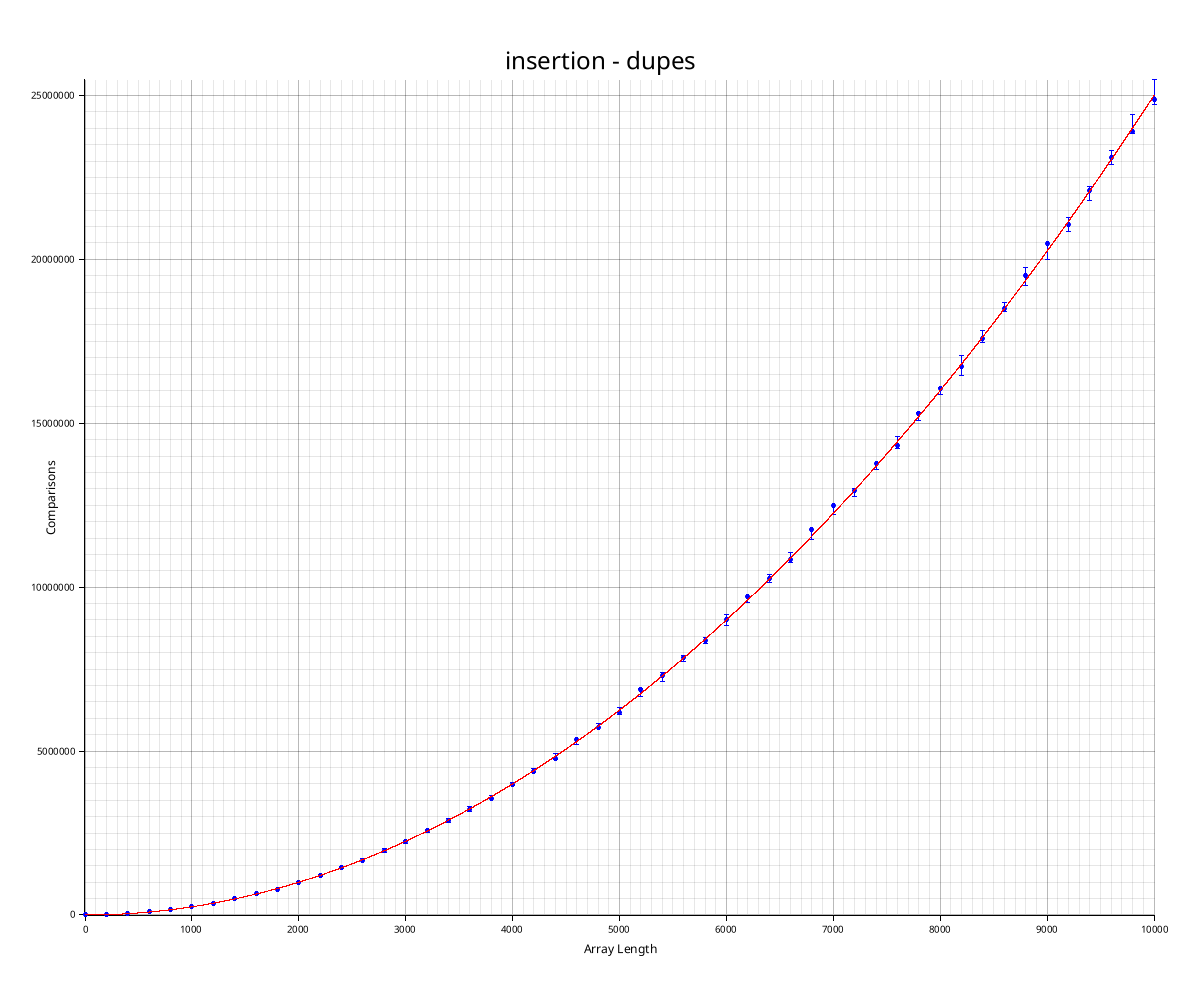
\includegraphics[width=\textwidth]{../plots/insertion-dupes.png}
    \caption{1/10th Unique Values}
    \label{fig:insertion-dupes}
  \end{subfigure}
  \begin{subfigure}[b]{0.5\textwidth}
    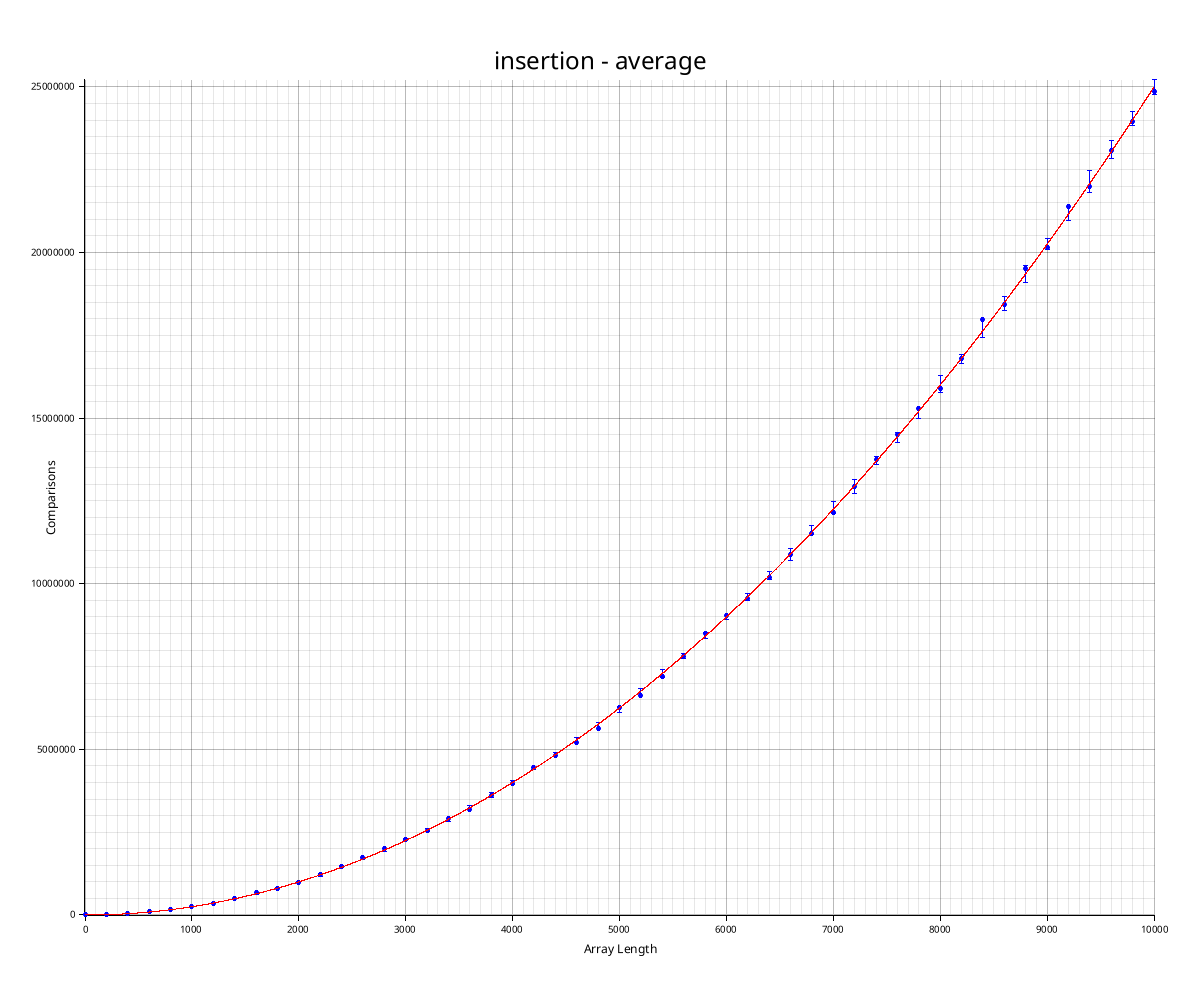
\includegraphics[width=\textwidth]{../plots/insertion-average.png}
    \caption{Average}
    \label{fig:insertion-avg}
  \end{subfigure}\hfill
\end{figure}

\section{Duplicate Values}
Insertion sort is getest op lijsten van lengte $n$ waarvan 1/5, 1/10, 1/20 en 1/40 van de waarden uniek zijn. 
In de grafiek \ref{fig:insertion-dupes} is de complexiteit van insertion sort te zien voor een lijst waarvan 1/10 van de waarden uniek zijn.
Met andere woorden elke waarde heeft nog 9 voorkomens in de lijst.
\par 
We merken op dat de complexiteit van insertion sort voor lijsten met duplicaten hetzelfde is als voor lijsten met unieke waarden.
Dit komt omdat insertion sort elke waarde vergelijkt en de grootste bijhoudt en vervolgens vanachter plaatst.
Omdat het algoritme niet weet dat er duplicaten zijn zal het algoritme nog altijd door de hele lijst moeten gaan om de grootste waarde te vinden.
\par
Het algoritme is voor elke lengte $n$ 10 keer uitgevoerd op een willekeurige lijst zoals hierboven beschreven.
We merken wel op dat de spreiding van de metingen dichter bij de theoretische complexiteit ligt dan bij lijsten met unieke waarden \ref{fig:insertion-avg}.
Dit komt omdat de lijsten met duplicaten minder variatie hebben in de volgorde van de waarden.
Er is meer kans dat elke waarde al op zijn plaats staat, in dit geval zijn er dan minder vergelijkingen nodig.

\section{Nearly Sorted}
Ik heb insertion sort ook getest op lijsten die bijna gesorteerd zijn. Elk element in de lijst is maximaal 5 plaatsen van zijn uiteindelijke plaats verwijderd.
Dit is gedaan door een gesorteerde lijst van lengte $n$ op te delen in subarrays van lengte 10 en deze subarrays te shuffelen.
\par
Elk element in de lijst is maximaal 5 plaatsen van zijn uiteindelijke plaats verwijderd.
Langs beide kanten kan een element dus 5 tot 0 plaatsen van zijn uiteindelijke plaats verwijderd zijn.
We hebben dus een totaal van 30 verplaatsingen en 10 mogelijke plaatsen voor elk element.
Nemen we dus het gemiddelde hiervan bekomen we $\frac{30}{10}=3$ gemiddelde verplaatsingen per element.

\begin{wrapfigure}{l}{0.5\textwidth}
  \begin{center}
    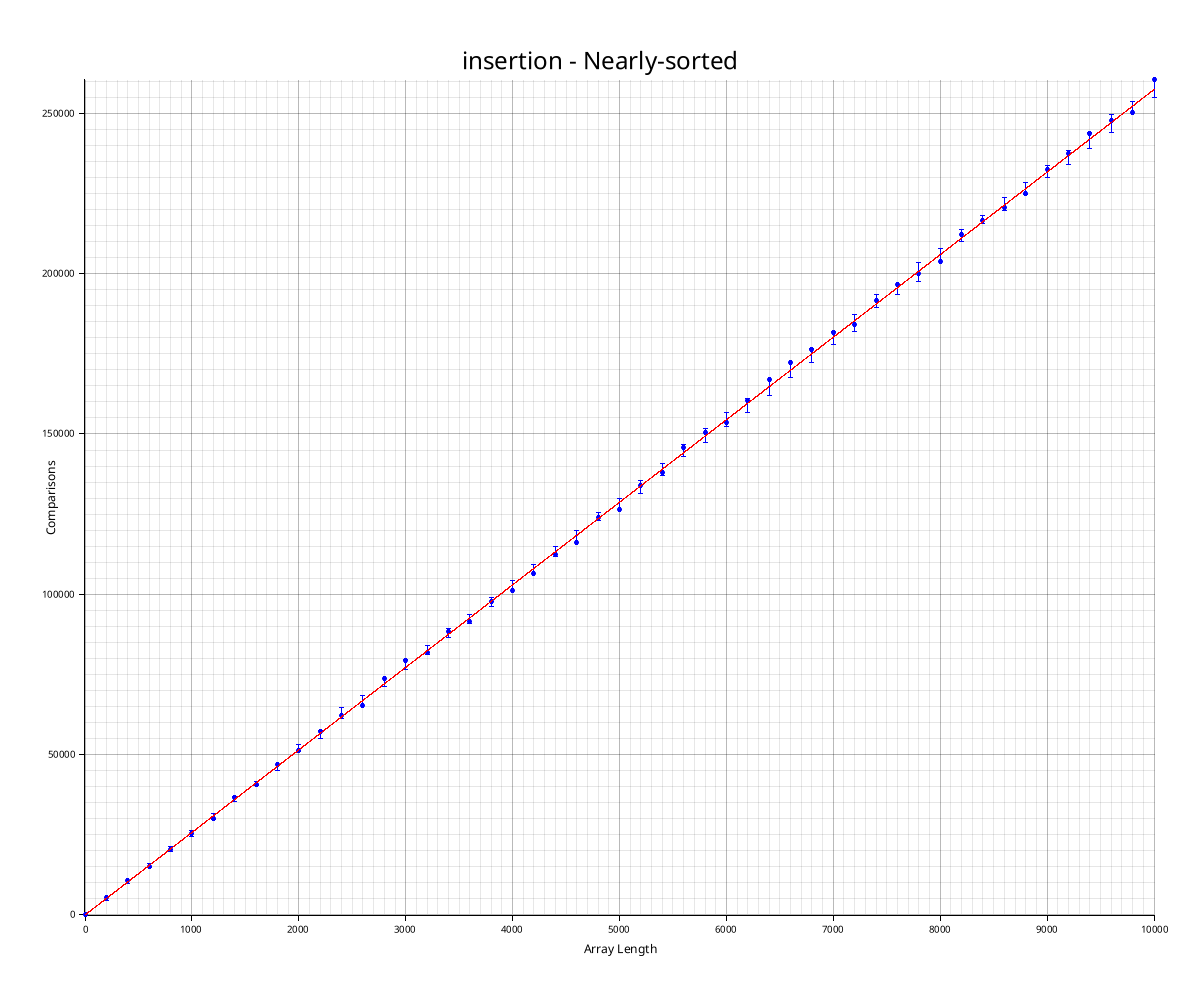
\includegraphics[width=0.48\textwidth]{../plots/insertion-nearly-sorted.png}
  \end{center}
  \caption{Nearly Sorted}
  \label{fig:insertion-nearly-sorted}
\end{wrapfigure}\hfill
\par
In de grafiek \ref{fig:insertion-nearly-sorted} is de complexiteit van insertion sort te zien voor een lijst die bijna gesorteerd is.
De rode lijn toont de theoretische complexiteit van insertion sort, namelijk $\sim 3n$.
De blauwe punten tonen de gemeten complexiteit over lijsten voor verschillende lengte $n$.
We merken dus op dat de gemeten complexiteit overeenkomt met de theoretische complexiteit.
\par
Voor lijsten die bijna gesorteerd zijn is de complexiteit van insertion sort dus $\sim kn$.
Waarbij $k$ de gemiddelde verplaatsingen per element is. In het geval voor \ref{fig:insertion-nearly-sorted} is $k=3$.
\par
Ook dit algoritme is voor elke lengte $n$ 10 keer uitgevoerd op een willekeurige lijst zoals hierboven beschreven.

\begin{wrapfigure}{r}{0.5\textwidth}
  \begin{center}
    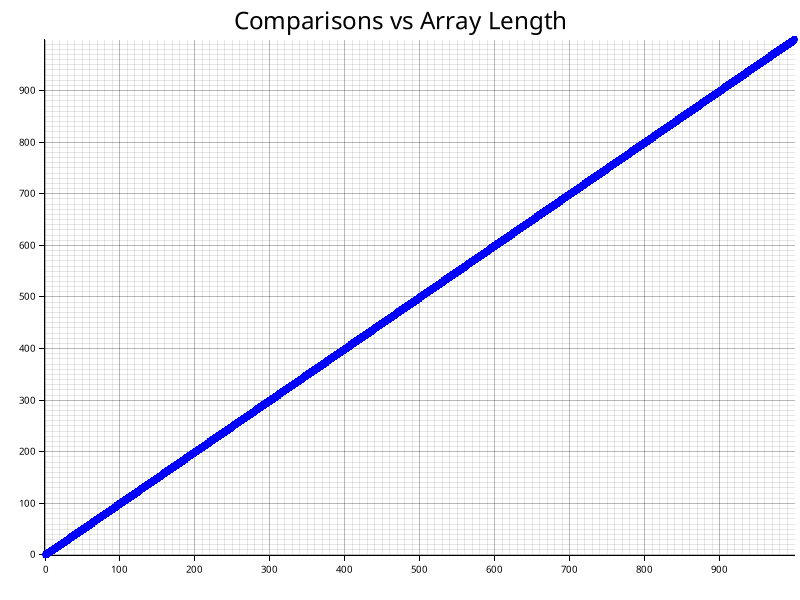
\includegraphics[width=0.48\textwidth]{../plots/insertion-best.png}
  \end{center}
  \caption{Best case}
  \label{fig:insertion-best}
\end{wrapfigure}

We merken op dat in tegenstelling tot insertion sort's best case scenario \ref{fig:insertion-best}, waar er geen spreiding is, er hier wel spreiding is.
Dit komt omdat de lijsten niet volledig gesorteerd zijn, en er dus nog steeds een variatie is in de volgorde van de waarden.

\end{document}